
\section{Material and methods}

\subsection{Simulation setup}

The monitoring system modeled in this simulation work is a Compton camera prototype under development within the French collaboration CLaRyS. The detectors detailed characteristics can be found in \cite{krimmer:hal-01101334}. A scheme of the simulation setup is given in figure~\ref{fig:fig_setup_CC_simulation_Hadronth}.

\begin{figure} [!hbtp]	
  \centering
  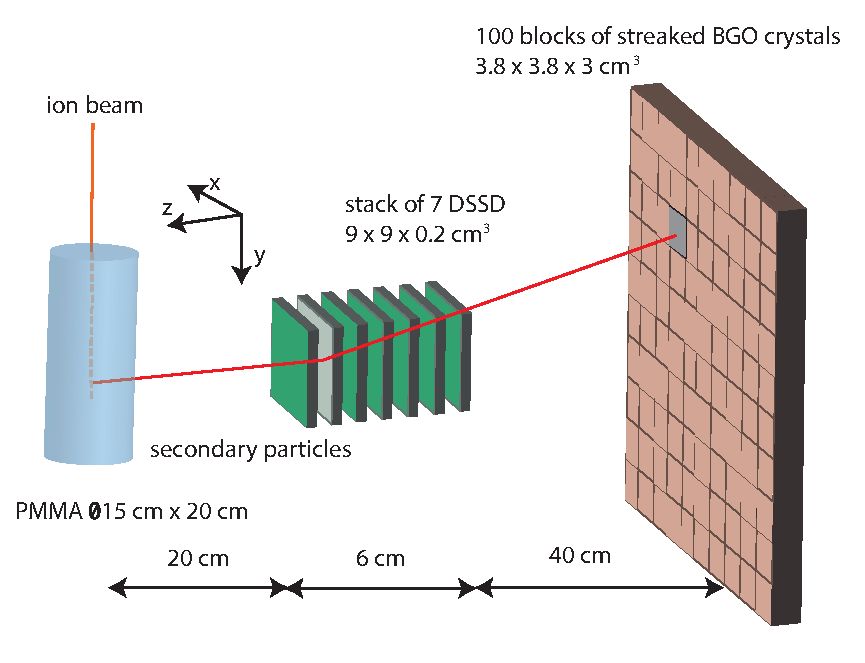
\includegraphics[width=0.7\textwidth]{./Figure/Compton_Camera_hadontherapy_PMMA_Cylinder_EN.pdf}
  \caption{Scheme of the simulation setup: a PMMA cylindrical phantom is set in front of the Compton camera prototype. The Compton camera is composed of a stack of 7 double sided silicon strip detectors (scatterer) and a plan of 100 single BGO blocks. The set distances are realistic for clinical conditions. This geometrical configuration has been used for all the simulations presented in this work.}
  \label{fig:fig_setup_CC_simulation_Hadronth}
\end{figure}

Like most of the Compton camera devices, the CLaRyS prototype includes a scatterer and an absorber. The scatterer consists of seven parallel planes of silicon detectors (double-sided silicon strip detectors, DSSDs), $9\times9\times0.2$~cm$^3$, with 1~cm distance between the centers of two neighboring planes, while the absorber is composed of an array of $10\times10$ BGO (Bismuth Germanate - Bi$_12$GeO$_20$) blocks ($3.5\times3.5\times3.0$~cm$^3$ each) placed at 40~cm from the last silicon layer (center-to-center distance). The ion beam interacts with a cylindrical PMMA (PolyMethylMethAcrylate) phantom (15~cm diameter and 20~cm length) placed in front of the Compton camera as target. It is placed 20~cm far from the first silicon plane (center-to-center distance) in order to fit with realistic clinical conditions.

The silicon detectors have a strip pitch of 1.4~mm, for a total of 64 strips per side (double-sided readout based on electron and hole pairs collection). The strips are not reproduced in the simulation code, and the transverse spatial resolution is set to 0.9~mm FWHM at the reference energy of 1~MeV, according to preliminary measurements performed on smaller detector prototypes. Concerning the parallel direction, the interaction position is set to the center of the involved silicon plane.

Regarding the BGO blocks, their entrance surface is streaked in a 8$\times$8 matrix of pseudo-pixels, 4.4~mm$^{2}$ side, and the readout is performed via 4 photo-multiplier tubes. The position reconstruction is achieved via Anger logic for the real detector, but a mono-block crystal is simulated here for simplicity. The events are selected to be limited to a single block component based on spatial analysis, and the interaction position is reconstructed via center of gravity calculation if multiple interaction occur. An incertitude contribution, randomly extracted by a Gaussian of 5~mm FWHM , is added to the reconstructed position to fit with the geometrical features. For what concerns the parallel direction, given the fact that the employed BGO blocks have not depth of interaction reconstruction capabilities, the interaction position is fixed to the center of the mono-block crystal.

Preliminary characterization measurements allowed to estimate the energy resolution of the BGO blocks, which is accordingly set to 17\% FWHM at the reference energy of 667~keV (a 137-cesium source has been used for the measurements). The energy resolution of the silicon detector is set to 2.3~keV (RMS) according to the design expectations; no characterization data are yet available for an instrumental estimate.

The time resolution has been set to 3.0~ns FWHM for the BGO blocks and to 15.0~ns FWHM for the silicon slabs, according to preliminary measurements performed on test detector modules at the GANIL %(Grand Accelerateur National d'Ions Lourds) 
center in France.

The detector resolutions play an important role in the Compton camera performances. The absorber spatial resolution influences the position of the apex of the Compton cone, as well as its axis orientation. The scatterer energy resolution determines the Compton cone aperture angle. The time resolution impacts the coincidence window between the absorber and the scatterer, and so its true/random coincidence discrimination capabilities.

The CLaRyS project also includes the development of a beam tagging hodoscope, composed of scintillating fibers read out by multi-channel photomultipliers. This detector is used to synchronize the beam time and space structure to the prompt gamma detection in order to tune the detection window reducing the background contamination. This detector section is not included in the simulation, but its time resolution has to be taken into account for the time-of-flight discrimination. It is set to 1~ns FWHM. The detectors spatial, energy and time resolutions are summarized in table \ref{table:table_resolution_detecteurs_CC_simulation_Hadronth}.

\begin{table} [!htbp]
\centering
%\begin{tabular}{>{\columncolor[gray]{0.9}}ccc}
\caption{Estimations of reachable resolutions with the detectors. Those resolutions are applied during the simulations.}
\begin{tabular}{cccc}
\hline
\textbf{Resolution (FWHM) at 1 MeV} & \textbf{Scatterer} & \textbf{Absorber} & \textbf{Hodoscope}\\
\hline 
\textbf{spatial [mm]	}			 &     0.9		 &  5 &	 1\\
%\hline
\textbf{energy}				&	2.3~keV		&  17~\%	&	/\\
%\hline
\textbf{timing [ns]}	        		&	15			&	3 	&  1\\
\hline
\end{tabular}
\label{table:table_resolution_detecteurs_CC_simulation_Hadronth}
\end{table}
    
The Monte Carlo simulation study is performed with the Geant4 toolkit, version 9.6 patch 02. Geant4 has been developed at CERN %(Conseil europ\'{e}en pour la recherche nucl\'{e}aire) 
for high energy physics experiments, but it has been shown that it can be used for ion beam therapy studies \cite{cirrone_hadrontherapy_2011,toshito_new_2010}. However, some improvements are still needed in order to extend the hadronic models to low energy applications~\cite{dedes_assessment_2014, Pinto:2016aa}.

The particle interactions in matter are described in this work by means of different models, listed in table~\ref{table:table_modele_physic_CC_simulation_Hadronth}. Additionally, the Doppler broadening and the photon polarization effects are taken into account.
 

\definecolor{Gray}{gray}{0.9}

\begin{table}[ht]
\label{physlist_ion}
\caption{Hadronic models used in the Geant4 simulations.}
\begin{scriptsize}
\begin{center}
\renewcommand{\arraystretch}{1.2}
%\begin{tabular} {>{\columncolor[gray]{0.9}}cccc}\hline  
\begin{tabular} {cccc}\hline
%\rowcolor{Gray}
\textbf{Process} & \textbf{Protons} & \textbf{Ions} & \textbf{Neutrons} \\ \hline 
\textbf{Electromagnetic} & \multicolumn{3}{c}{standard$_{\rm{option3}}$} \\ %\hline
\textbf{Inelastic} & G4BinaryCascade & G4QMDReaction  &  G4BinaryCascade  \\ 
 & & (G4IonsShenCrossSection)&+ G4NeutronHPInelastic ($<$19 MeV)\\ %\hline
\textbf{Elastic} & G4LElastic & G4LElastic & G4LElastic + G4NeutronHPElastic ($<$19 MeV)\\ %\hline
\textbf{Fission} & / & / & G4LFission + G4NeutronHPFission($<$19 MeV) \\ %\hline
\textbf{Capture} & / & / & G4LCapture +  G4NeutronHPCapture ($<$19 MeV) \\ %\hline
\textbf{Radioactivedecay} & / & G4Radioactivedecay & / \\ \hline
\end{tabular}
\end{center}
\end{scriptsize}
\label{table:table_modele_physic_CC_simulation_Hadronth}
\end{table}

The two main beam particles used in clinics are considered in this work: protons and carbon ions. The beam range of interest is 15.2~cm in the PMMA phantom, and the associated energy is 160~MeV for protons and 305~MeV/n for carbon ions.
 
In order to reproduce a realistic clinical beam, the beam transverse dimension is modeled with a Gaussian distribution with a standard deviation of 5~mm for protons at 160~MeV and 3.5~mm for carbon ions at 305~MeV/n. The Compton camera setup does not change for the different incident particles. The beam intensity for a spot in pencil beam scanning (PBS) mode for protons is $10^8$~particles and $10^5$~particles for carbon ions. The beam time structure is applied in the data analysis stage, described below.\newline

\subsection{Data treatment}
\label{subsection:Treatment_data_CC_hadrontherapy_Geant4}

\subsubsection{Time structure and treatment}
\label{subsubsection:modelisation_fasceau_ions_CC_hadrontherapy_Geant4}
 
Two different beam time structures have been considered for this study, related to two kinds of accelerators used in clinical practice: the IBA C230 cyclotron for protons (used in 16 clinical centers worldwide) and the Heidelberg (Germany) synchrotron installed in the Ion Therapy Center (HIT) for carbon ions. Even if the beam microstructure changes depending on the ion energy and the beam intensity, the microstructure is modeled according to the reported features at a specific energy and intensity for simplicity. For protons at 160 MeV, the primary particles are grouped in bunches of 2~ns (this value may vary also according to the distance between the cyclotron and the treatment room, and energy spread selection) at a frequency of 106~MHz (9.42~ns)~\cite{f_roellinghoff_real-time_2014}. The clinical beam intensity is 3.2~nA which corresponds to about 200 protons per bunch. Concerning the carbon ion beam at 305~MeV/u, the estimated microstructure is composed of 30~ns duration bunches at a frequency of 5.9~MHz (170~ns period). The clinical beam intensity for carbon ions is $5\times10^7$~ions/s, corresponding to about 9~ions per bunch. This beam structure is extrapolated from measurements performed by our group in 2013 at HIT; the beam time structure was measured for 200~MeV/u and 400~MeV/u primary ion energy with a two-fiber hodoscope (basic prototype of the one at present under development) and the spill signal was given by the accelerator. Figure \ref{fig:fig_structure_temps_faisceau_HIT_2013_CC_simulation_Hadronth} shows the beam structure for carbon ions at 400~MeV/u. The pulses have a spill period of 150.2~ns and each bunch is approximately 21.5~ns.
The mentioned measurements have shown that the spill phase changes during the extraction: this implies that the HF signal from the synchrotron can not be used to trigger the pulses, so that the use of an additional beam time stamp system like the hodoscope seems required for time-of-flight background rejection purposes.\newline

	\begin{figure} [!hbtp]	
	\centering
	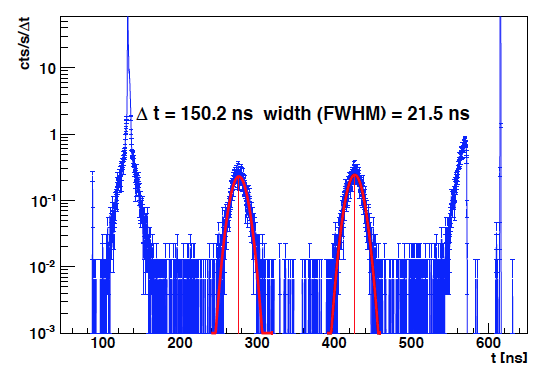
\includegraphics[width=0.5\textwidth]{./Figure/2013_Structure_Time_Beam_400MeV.png}
	\caption{Time micro-structure measured from a carbon ion beam at 400~MeV/u delivered at HIT. The pulses have an extraction period of 150.2~ns and the bunches are 21.5~ns FWHM. The measurement was achieved with a two-scintillating-fiber hodoscope.}
	\label{fig:fig_structure_temps_faisceau_HIT_2013_CC_simulation_Hadronth}
	\end{figure}


The coincidence window (between scatterer and absorber events) is set to 40~ns, centered on each absorber detected interaction. This value is adapted to the detectors time resolutions. Table~\ref{table:definition_beam_structure_CC_hadrontherapy_Geant4} summarizes the presented beam time structures and coincidence reconstruction features.

\begin{table} [!htbp]
\footnotesize
\centering
\caption{Description of the two beam structures studied: the IBA cyclotron C230 for protons and the synchrotron installed at the Heidelberg Ion Therapy Center (HIT) in Germany for carbon ions. The macro-structure of the synchrotron, at the second time scale, is not considered here. The beam structures are applied to the simulation data.}
\setlength{\tabcolsep}{2pt}
%\hspace{-2.1cm}
\begin{tabular}{c>{\columncolor[gray]{0.9}}ccc}
\cline{2-4}
%\hline
		\multicolumn{2}{c}{ }		 & 					\textbf{Protons} & \textbf{Carbon ions}\\ 
%\hline
\cline{2-4}%\hline
\multirow{3}{*}\textbf{Clinical features}		&	\textbf{Facility}	& IBA Cyclotron C230&   Synchrotron at HIT\\
											& \textbf{Clinical intensity}& $  2\times10^{10}$ p/s  & $  5\times10^{7}$ ions/s\\
											& \textbf{Energy} 			&160 MeV 			&    305 MeV/u\\
\cline{2-4}%\hline
\multirow{3}{*}\textbf{Beam structure}		&	\textbf{Bunch time [ns]}			& 3.2				&  30\\
											& \textbf{Period [ns]}		&   9.4 				& 170\\
											& \textbf{Primaries  /bunch} 	&217 			& 9\\
\cline{2-4}%\hline
\multirow{2}{*}\textbf{Detectors}						& \textbf{Coincidence window [ns]}		& 40 	&  40 \\
											&\textbf{Time resolution [ns]} & \multicolumn{2}{c}{Si: 15 and BGO: 3}\\
\cline{2-4}%\hline
\end{tabular}
\label{table:definition_beam_structure_CC_hadrontherapy_Geant4}
\end{table}



\newpage
%---------------------------------------------------------------
%---------------------------------------------------------------
\subsubsection{Data selection: time and energy cuts}
\label{MatMeth::TOF_Ecut}

As already explained in the introduction, the Compton detection principle is based on a double interaction in the scatterer and absorber section, where an interaction is defined as an energy deposit in a detector module. As discussed in section~\ref{subsubsection:modelisation_fasceau_ions_CC_hadrontherapy_Geant4}, the coincidence reconstruction relies on a defined time window, fixed according to the involved detector resolution. In a simulation environment, different kinds of coincidences events can be distinguished and studied: 
\begin{itemize}
\item[-] real coincidences: created by a single photon first interaction in a single scatterer plane and then in a single absorber block;
\item[-] quasi-simultaneous interaction from two secondary particles;
\item[-] double interaction from the same particle different from a gamma.
\end{itemize}

In a real clinical environment there is no way to select the real coincidences, so that the collected data are affected by a certain number of the so-called random coincidences. The amount of random coincidences depends on the detector time resolutions, on the fixed time coincidence window and on the beam time structure, for fixed beam energy, phantom composition and camera prototype setup. In figure~\ref{fig:fig_explication_coincidence_CC_simulation_Hadronth} a schematic view of the different kinds of coincidences is presented.

\begin{figure} [!hbtp]	
  \centering
  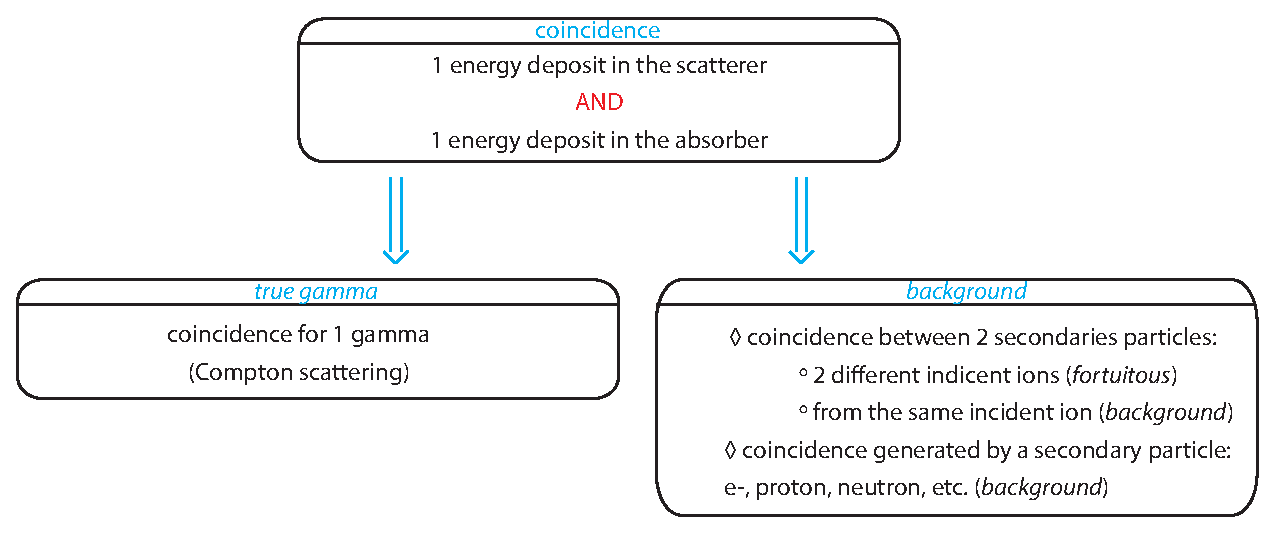
\includegraphics[width=0.9\textwidth]{./Figure/Schema_coincidence_EN.eps}
  \caption{Diagram showing the different definitions of coincidences in the Compton camera.}
  \label{fig:fig_explication_coincidence_CC_simulation_Hadronth}
\end{figure}

In addition to this, the prompt gamma measurement is contaminated by other secondary particles produced by the beam interaction with the patient/phantom, mainly massive and charged particles (protons, neutrons). 
As already mentioned, it has been demonstrated by our group that a time-of-flight discrimination is possible and effective in reducing this source of background. In fact, the photons are moving at the speed of light while the massive particles approach the detector at a lowest speed. The time information coming from the hodoscope and from the absorber can be then combined to fix a detection time window and reject all the events outside the window. In this work, the time between the incident particle creation and the secondary particle detection in the absorber is considered as the time-of-flight. The hodoscope time resolution $u_{hodoscope}$ (1~ns FWHM) is applied to the primary particle creation time, with a contribution randomly extracted from a Gaussian with $\sigma\,=$ 1/2.35~ns, while the detection time in the absorber is affected by the absorber time resolution.

 \begin{eqnarray}
TOF_{theoretical} = t_{absorber}-t_{hodoscope} \\
TOF_{simulation} = t_{absorber}+t_{creation} + u_{hodoscope}
\label{TOF_equation}
\end{eqnarray} 

The time-of-flight spectrum resulting from the simulation shows that the coincidences of interest (produced by prompt-gamma rays) are included in a window between 0 and 6~ns (figure \ref{fig:fig_TOF_distribution_CC_simulation_Hadronth}). Therefore, all the coincidences with a TOF higher than 6~ns have been rejected, reproducing a possible clinical background rejection scenario. 

\begin{figure} [!hbtp]	
  \centering
  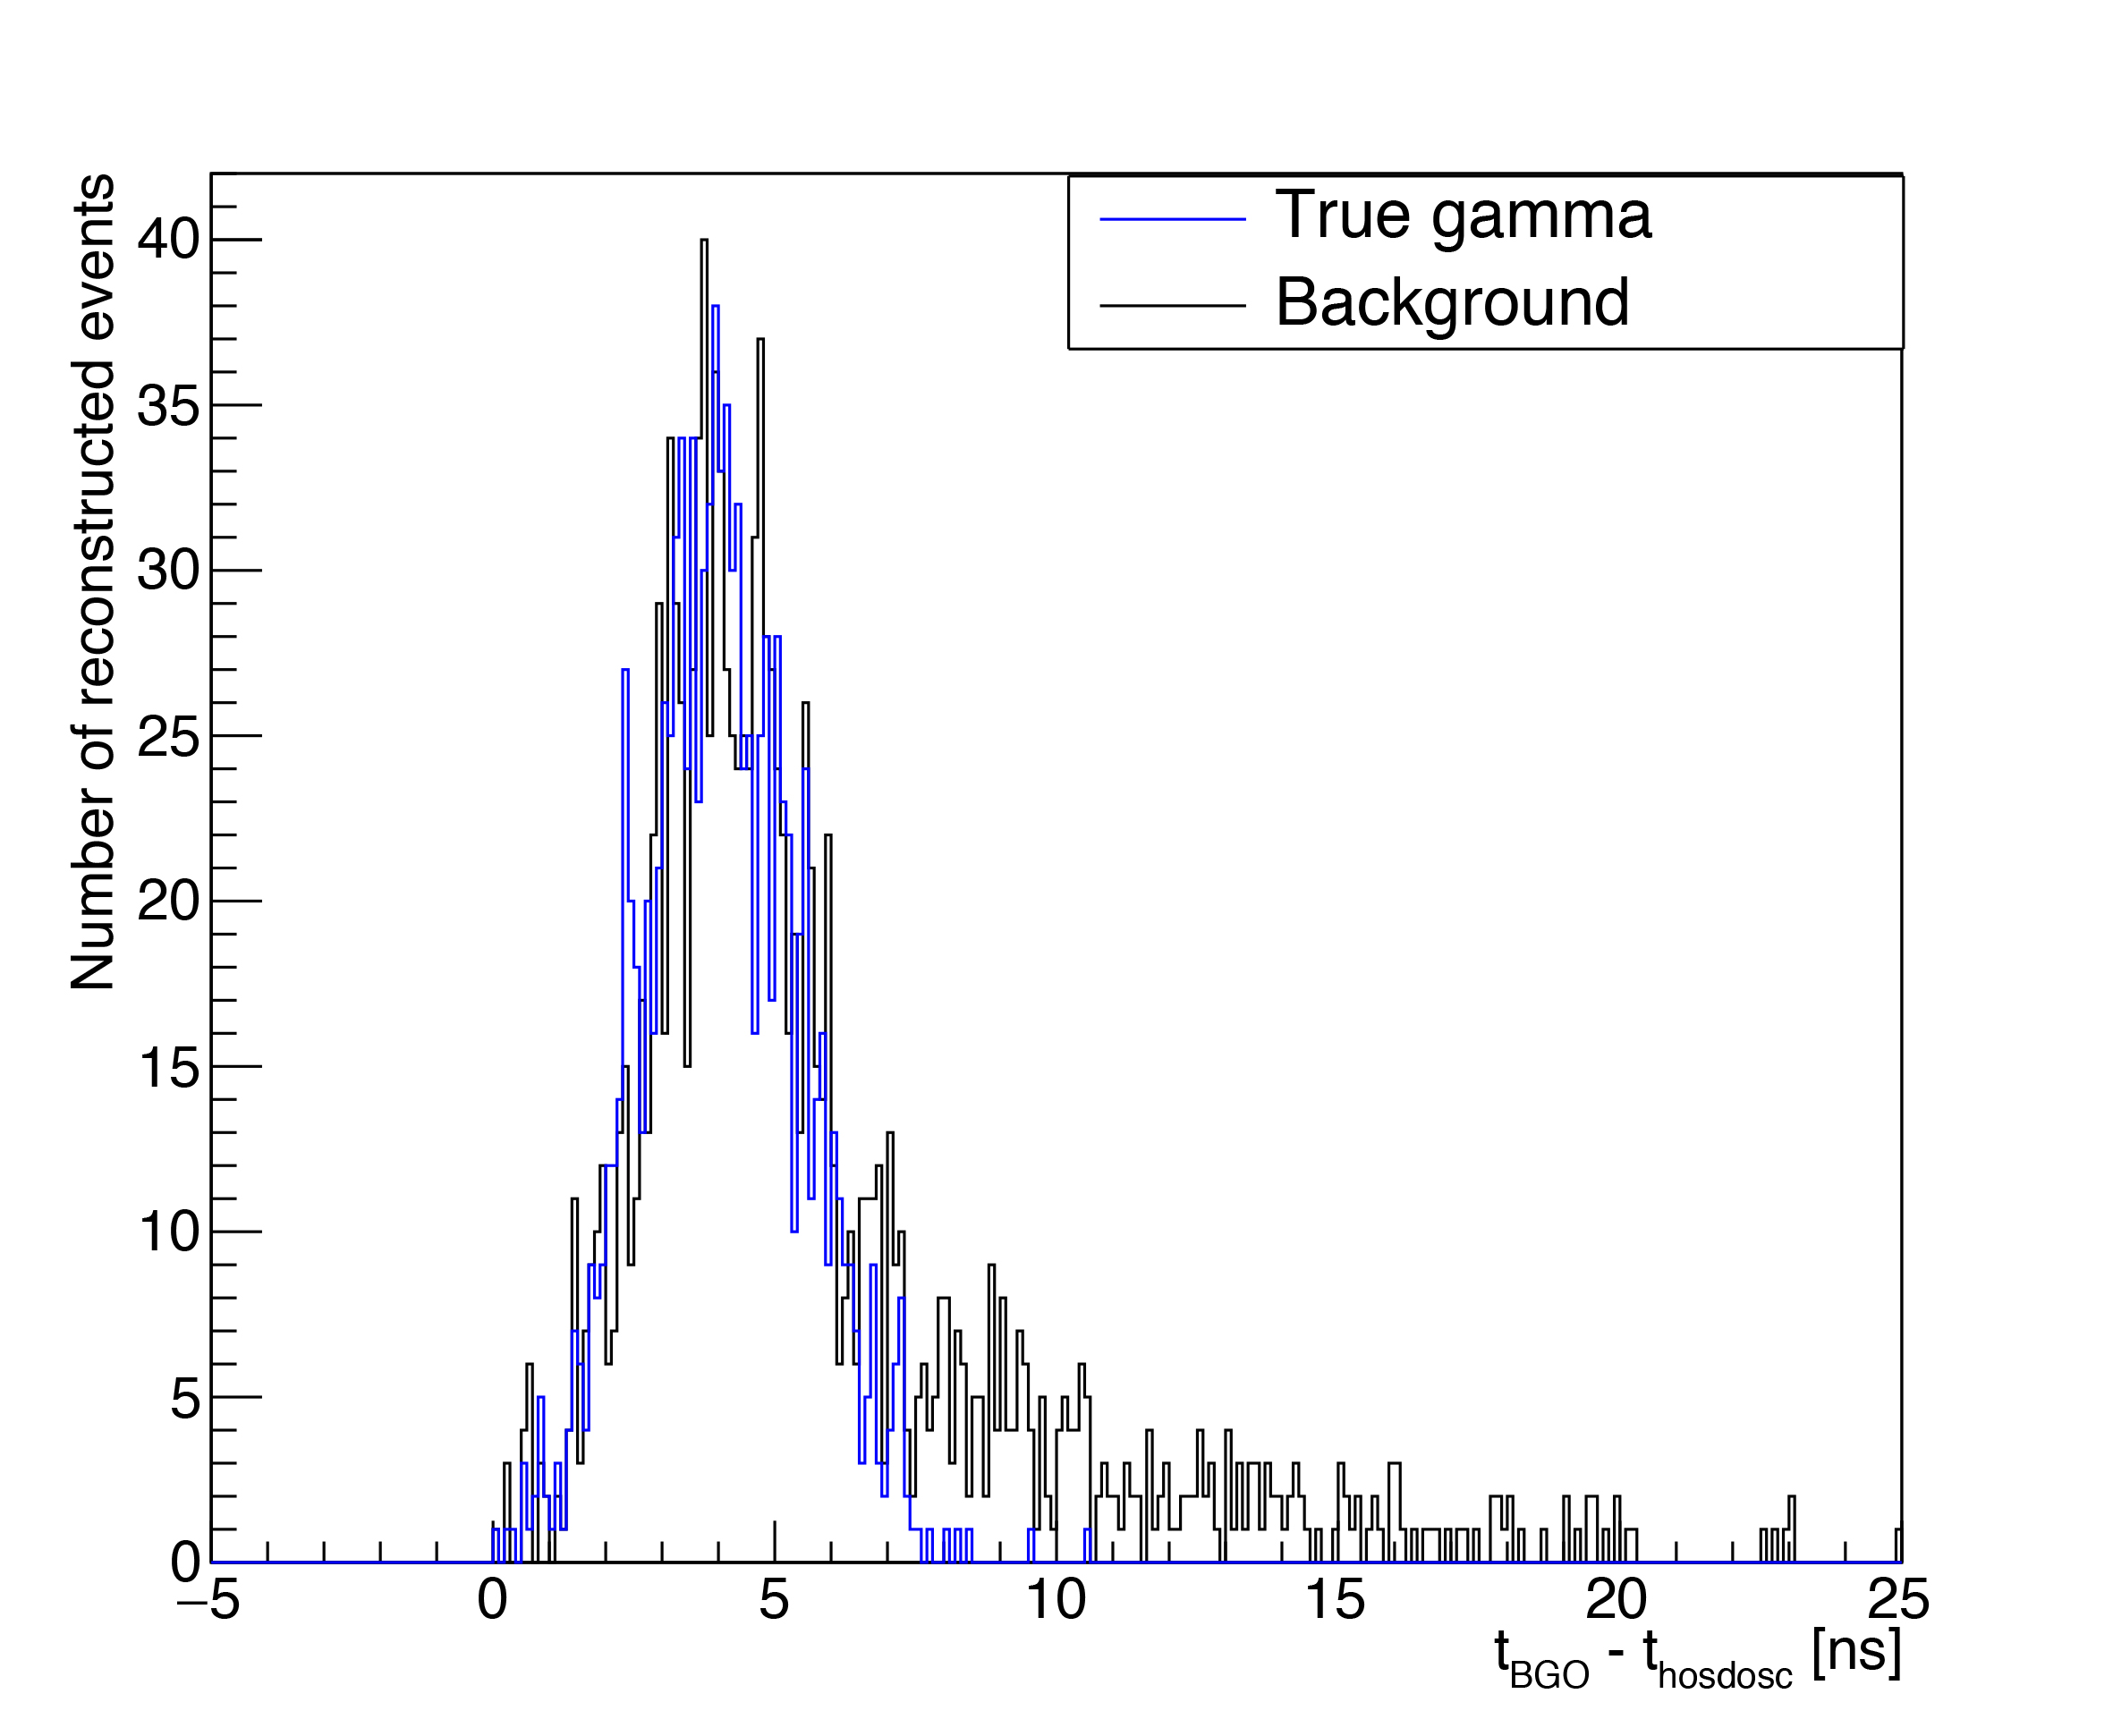
\includegraphics[width=0.6\textwidth]{./Figure/2015_01_04_TOF_spectra_NoCut_1Proton_ResolTemporelle_applied_these.jpg}
  \caption{Time of flight spectrum obtained by means of the simulation for a proton beam at 160 MeV and $1\times10^{8}$ incident protons. The detection time for the absorber is given by the tag for the first deposit energy. The blue curve represents the time of flight for true events and the black one represents the background.}	
  \label{fig:fig_TOF_distribution_CC_simulation_Hadronth}
\end{figure}

In addition to the time-of-flight based selection, energy thresholds are also defined for the event detection. On a single detector basis, 50~keV is set as lower threshold for the silicon layers and 100~keV for the absorber. On a complete event basis, a total absorbed energy lower limit is set to 1~MeV.

\subsection{Reconstruction algorithm}

Once the coincidences are defined and selected according to the fixed physical cuts, the prompt-gamma emission point has to be reconstructed for each event. This can be done via analytic or iterative algorithms based on the Compton kinematics (see section~\ref{section::Intro}), presented in the following sections.


\subsubsection{Line-cone algorithm}
The reconstruction via line-cone algorithm exploits the energy deposit and position information collected by the camera in addition to the beam path information. Thanks to the deposited energies in the detectors and the interaction positions, a cone surface is analytically defined via the Compton equation~\ref{Compton_equation}.
\newline
We assume that the initial energy of the gamma ray is fully absorbed in the absorber. This hypothesis, combined to the detector energy resolutions, leads to a potential uncertainty on the cone aperture. The interaction position in the scatter gives the cone apex and the line connecting the interaction position in scatterer and absorber gives the cone axis. In order to simplify the reconstruction, the beam direction is used to limit the possible solutions (laying on the reconstructed cone surface) to two points (intersection of the beam direction and the reconstructed cone). The set of all the reconstructed points gives the emission source distribution. The obtained final image is then the 2 dimensional projection of the prompt gamma emission spectrum. 

\subsubsection{LM-MLEM algorithm}	

The iterative methods allow to get a 3D image reconstruction, potentially by taking into account the spatial resolution and the energy resolution of the detectors. Few iterative algorithms have been developed for Compton event reconstruction. \cite{schone_common_2010, zoglauer_design_2011,gillam_compton_2011,mackin_evaluation_2012,lojacono_low_2013}.

The \textit{List-Mode Maximum Likelihood Expectation Maximization} (LM-MLEM) algorithm is a MLEM version which allows to free from sinograms and to reconstruct the image directly from the list of detected events.
The first step is to define the volume which includes the origin of the prompt gamma ray detected. This volume is divided into equal voxels and the emission intensity is assumed homogeneous for each voxel $j$, with a Poisson distribution of parameter $\lambda_j$ (a vector of the emissions intensities of all the voxels). The algorithm is based on a system matrix $T$ composed of the coefficients  $t_{ij}$ which represent the probability that a photon produced in the voxel $j$ is detected in coincidence by the Compton camera as an event $i$. The probability for a gamma detected in coincidence to be emitted from the voxel $j$ is denoted as $s_j$.
The LM-MLEM algorithm starts with an initial value $\lambda^{(0)}$, which can be the simple back-projection reconstruction.
The iterations rely on the following recurrence relation:

\begin{equation}
\lambda_j^{(l+1)} =  \frac{\lambda_j^{(l)} }{s_j} \sum\limits_{i=1}^{N_{\gamma}} t_{ij} \frac{1}{P_i^{(l)}},\quad \rm{with}\quad  P_i^{(l)}=\sum\limits_{k=1}^{N_{v}} t_{ij}\lambda_k^{(l)},
 \label{eq:equation_lambda_compton_med_nucleaire}\newline
\end{equation}
where $N_{\gamma}$ is the number of detected events and $N_v$ is the number of voxels in the image.\newline

The LM-MLEM algorithm used for this study is the one developed by the CREATIS research group in Lyon~\cite{maxim_filtered_2014,hilaire_compton_2014}.\newline%\cite{maxim_analytical_2009,lojacono_low_2013,maxim_filtered_2014,hilaire_compton_2014}.\newline
For each photon detected, the system matrix $T$ is calculated by taking into account the uncertainties on the angle between the source and the involved scatterer plane and the angle between the scatterer plane and the absorber involved module.
The matrix elements $t_{ij}$ are calculated as:
\begin{equation}
 t_{ij} = K(\beta_i,E_{tot})\frac{|\rm{cos}(\theta_{\overrightarrow{V2V1})} |}{V_2V_1^2} \int\limits_{M\in v_j} \frac{|\rm{cos}(\theta_{\overrightarrow{V_1M})}| }{V_1M^2} h_i(M)dv,
 \label{eq:equation_tij_compton_med_nucleaire}\newline
\end{equation}
where $\beta_i$ is the Compton scattering angle, $V_1$ the interaction position in the scatterer, $V_2$ the interaction position in the absorber, $h_i$ the spatial kernel which models the uncertainties on the Compton angle for each voxel $M$, $K(\beta_i,E_{tot})$ the differential cross section and $v$ the reconstructed volume.\newline

In order to simplify and speed up the calculation of the $t_{ij}$ matrix, the voxels located far from the reconstructed cone are set to 0. The distance between the cone and the voxel is calculated by taking the voxel center as reference point. The spatial resolutions are not included in this version of the algorithm.\newline
For each iteration, the matrix $T$ is stored and the reconstructed image can be produced via a Matlab simple interface.

\subsection{Precision estimation}
\label{MatMeth:precision}

The camera precision is defined as the difference between the expected Bragg peak position (according to the treatment planning) and the Bragg peak position reconstructed through the data. This is a critical parameter which will be used to fix a decision threshold during a ion beam treatment.
 
In this study a reference profile has been defined as the reconstructed emission vertex profile at high statistics, via analytic (line cone) and iterative (LM-MLEM) algorithms; this will be used to mimic the treatment planning. This Bragg peak position is compared to the ones reconstructed at lower statistics (close to clinical conditions) via analytic and iterative algorithms.

The high statistic profile has been obtained with $2\times10^{10}$ incident protons (figure~\ref{fig:fig_Results_Estimation_Camera_Profil_highStat_CC_simulation_Hadronth_LineCone}) for the line-cone reconstruction and with $1\times10^{10}$ incident protons (figure~\ref{fig:fig_Results_Estimation_Camera_Profil_highStat_CC_simulation_Hadronth_MLEM}) for the LM-MLEM reconstruction method. The \textit{SmoothKern} method, with the Nadaraya-Watson regression, is used to smooth the reference profiles in order to reduce relative statistic fluctuations.\newline
A region of interest (ROI) ranging from $y=0$ mm to $y=+100$ mm is defined around the expected Bragg peak position, located at $y=+50$~mm in the phantom. The reference profiles are modelled in the ROI by a linear combination named Non-Uniform Rational Basis Splines (NURBS). \newline
A new independent profile should be simulated at low statistics for the precision calculation. However, with the aim to speed up the analysis, a random extraction from the NURBS profile (\ref {fig:fig_Estimation_Camera_CC_NURBS_Poisson_LC} and \ref {fig:fig_Estimation_Camera_CC_NURBS_Poisson_MLEM}) is performed following the Poisson law, in order to select reduced data sets. The desired low statistics ranges from $10^8$ to $5\times10^9$ incident protons.\newline
The minimal distance between the NURBS reference profile and the low statistic reconstructed profiles is estimated thanks to the $\chi^2$ method. For the $\chi^2$ estimate, the low statistics profile is defined around the fall-off position from $y=+30$ mm to $y=+70$ mm. The minimization process tests the profiles at low statistics on a 60 mm variation range, between $-30$~mm and $+30$~mm with respect to the initial position, with a step of $0.1$~mm. The      $\chi^2$ is calculated as follows:

\begin{eqnarray}
\chi^2 = \sum\limits_{i=1} {(y_{sample,i}-y_{NURBS,i})^2},
\end{eqnarray}

where $y_{sample}$ is the number of coincidences for the low statistics profile, $y_{NURBS}$ is the number of coincidences for the reference profile NURBS (scaled at the same low statistic) and i the step number.\newline
The global minimum of all the reconstructed profiles is then retrieved. The figures \ref{fig:fig_Results_Chi2_Distribution_Variation_CC_simulation_Hadronth_LC} and  \ref{fig:fig_Results_Chi2_Distribution_Variation_CC_simulation_Hadronth_MLEM} show the distribution of $\chi^2$ calculated for a low statistic profile at $10^8$ incident protons.\newline
A total of a thousand profiles at the low statistic are generated (named realizations) and the $\chi^2$ minimization is applied to each of them. The standard deviation of the distribution resulting of the thousand results gives the precision of the camera for a given number of incident protons. The figure~\ref{fig:fig_Results_Precision_Distribution_Variation_CC_simulation_Hadronth_LC} and~\ref{fig:fig_Results_Precision_Distribution_Variation_CC_simulation_Hadronth_MLEM} show the distributions at $10^8$ incident protons for the line-cone and LM-MLEM algorithms.


\begin{figure} [!h]
\subfloat[\label{fig:fig_Results_Estimation_Camera_Profil_highStat_CC_simulation_Hadronth_LineCone}]{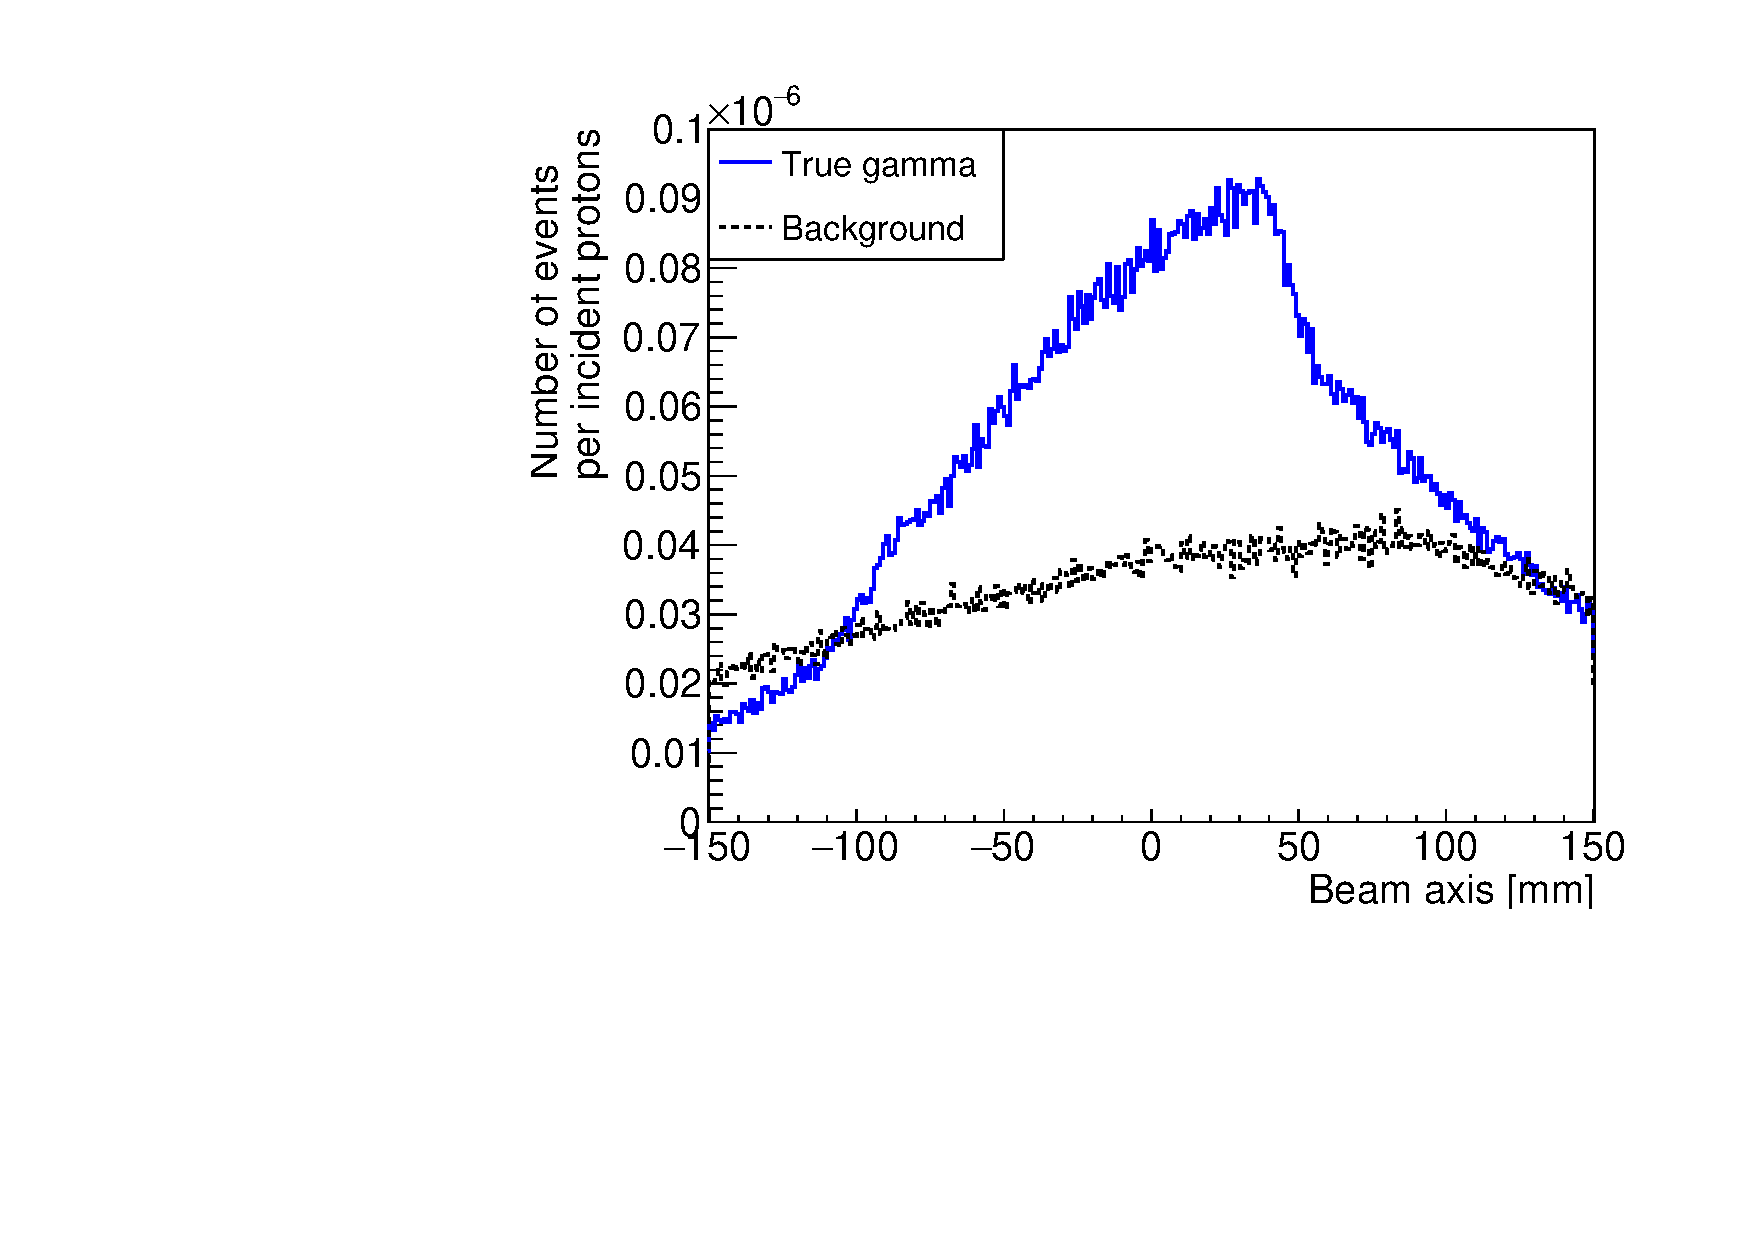
\includegraphics[width=0.33\textwidth]{./Figure/profile_high_stat_linecone.pdf}}
\subfloat[\label{fig:fig_Results_Estimation_Camera_Profil_highStat_CC_simulation_Hadronth_MLEM}]{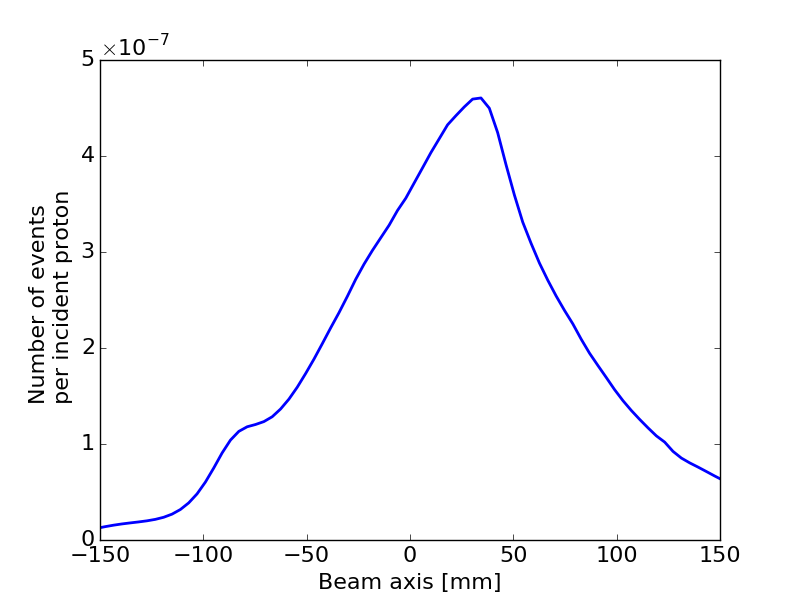
\includegraphics[width=0.32\textwidth]{./Figure/profileY_corr_r15.png}}\\
 %\subfloat[\label{fig:fig_Estimation_Camera_CC_NURBS_Poisson_LC}]{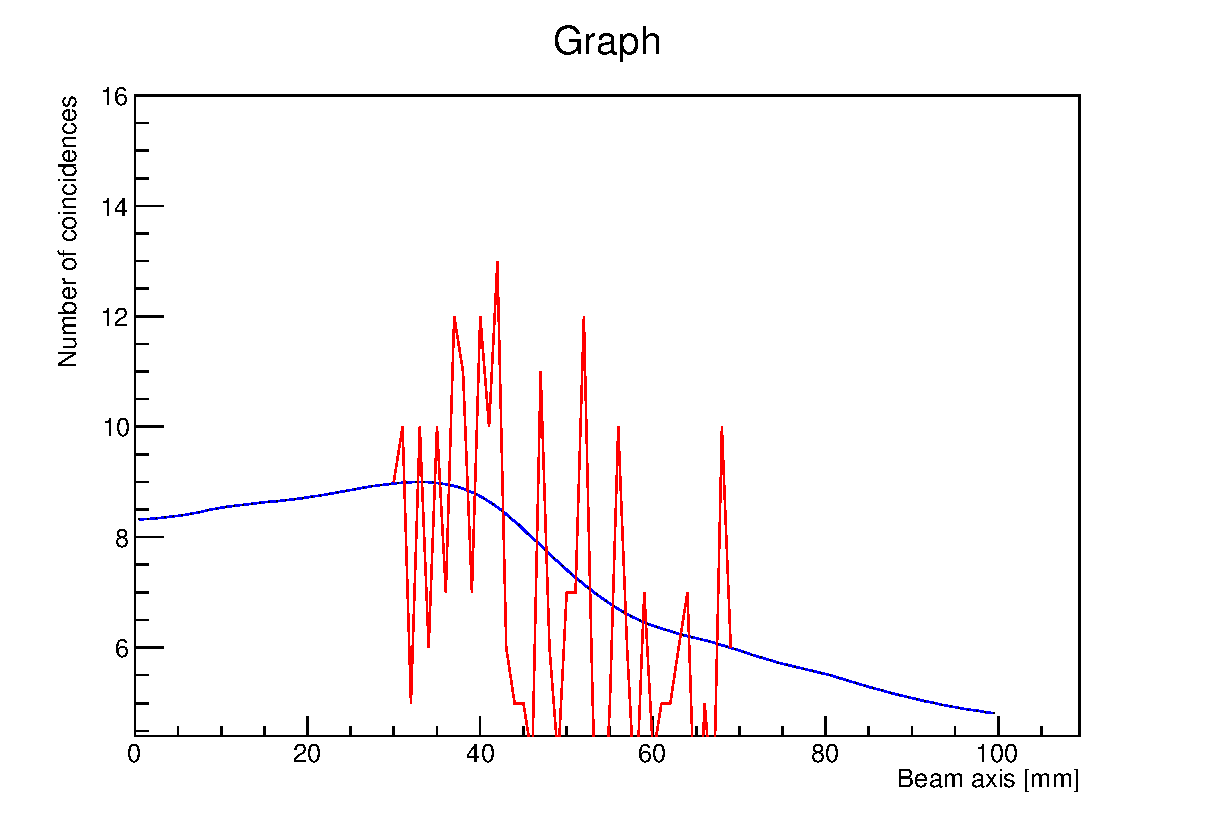
\includegraphics[width=0.33\textwidth]{./Figure/2017-08-02_Poisson_Nurbs_1e8_Article_LC.eps}}
 \subfloat[\label{fig:fig_Estimation_Camera_CC_NURBS_Poisson_LC}]{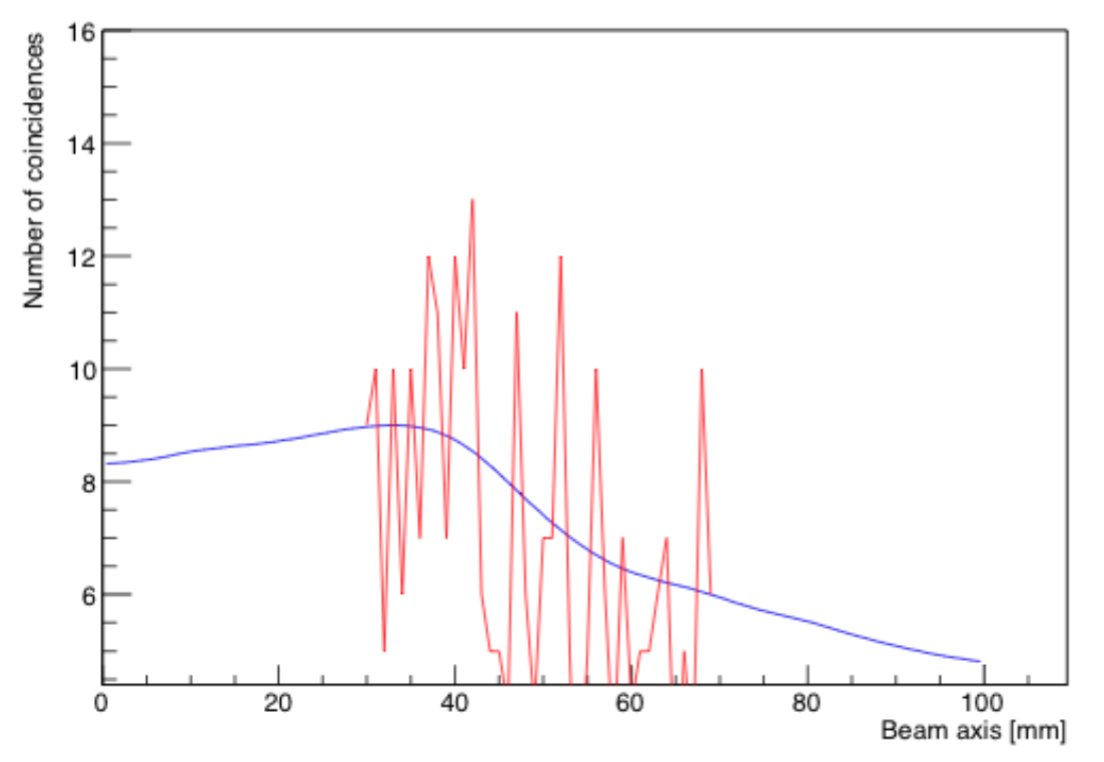
\includegraphics[width=0.33\textwidth]{./Figure/line_cone_NURBS.png}}
 %\subfloat[\label{fig:fig_Estimation_Camera_CC_NURBS_Poisson_MLEM}]{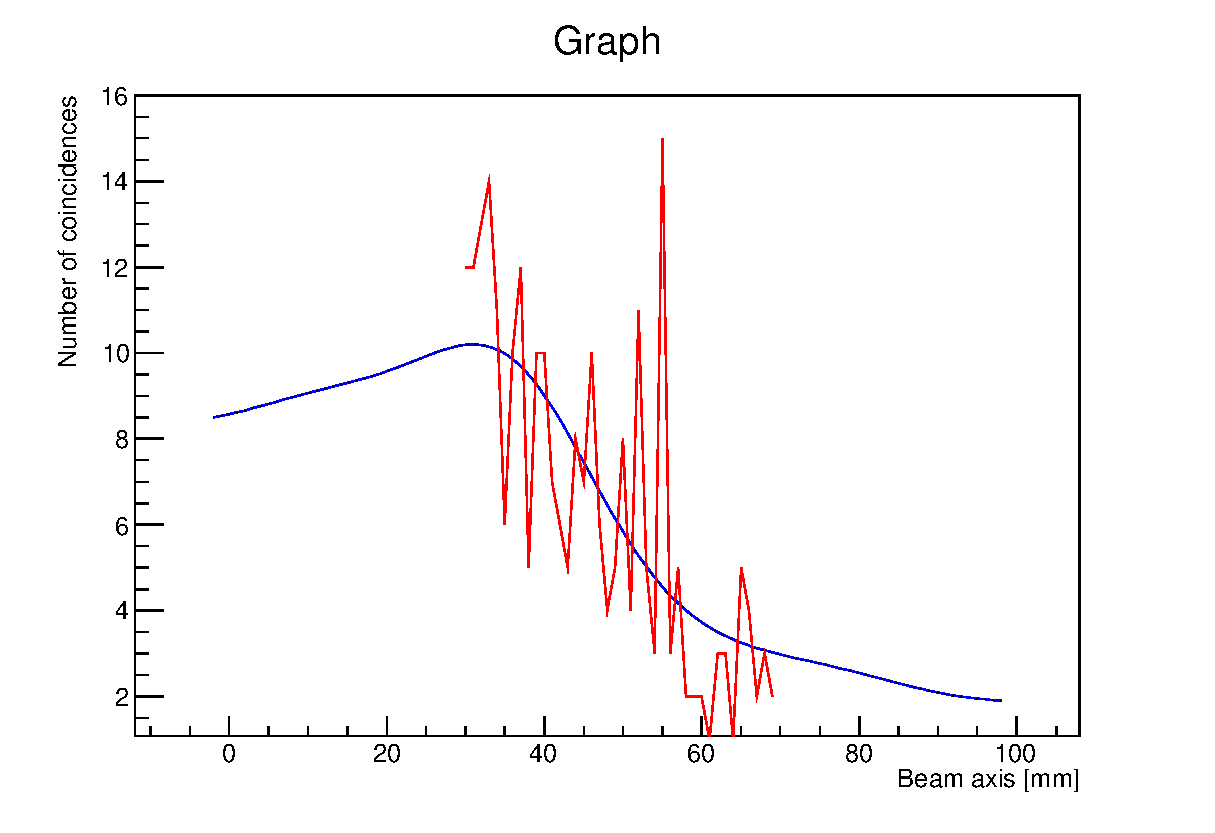
\includegraphics[width=0.33\textwidth]{./Figure/2017-08-02_Nurbs_Poisson_1e8_Article_MLEM.eps}}\\
 \subfloat[\label{fig:fig_Estimation_Camera_CC_NURBS_Poisson_MLEM}]{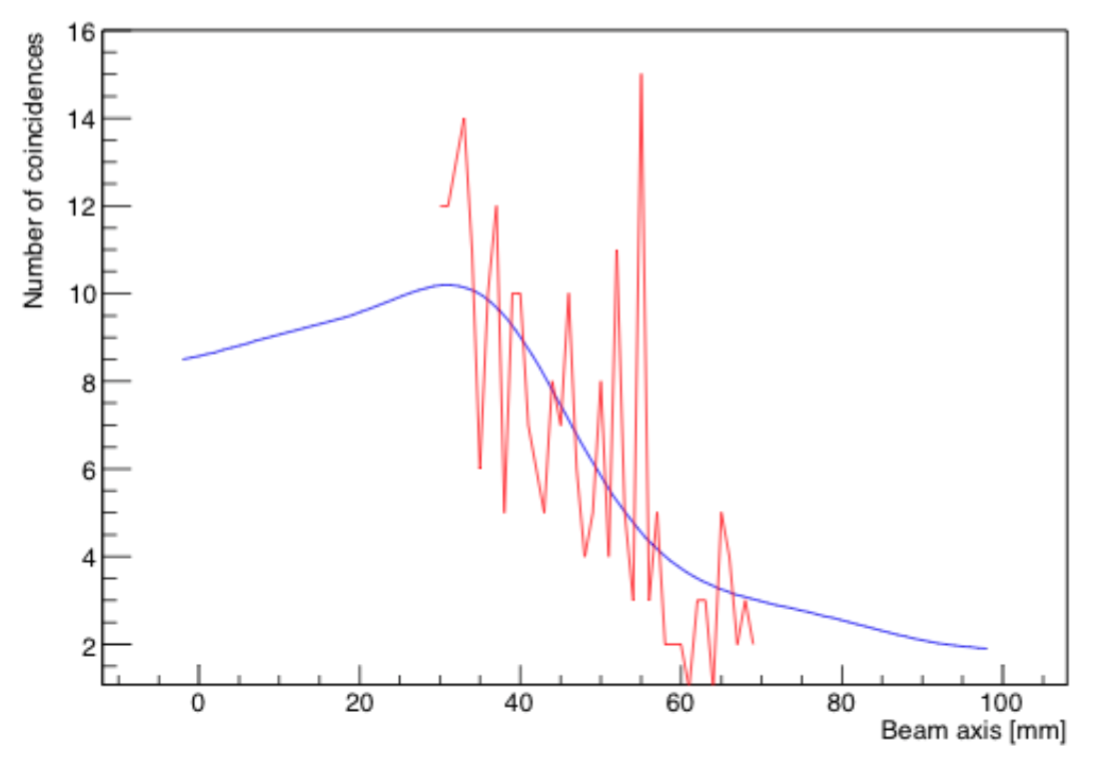
\includegraphics[width=0.33\textwidth]{./Figure/MLEM_NURBS.png}}\\
  %\subfloat[\label{fig:fig_Results_Chi2_Distribution_Variation_CC_simulation_Hadronth_LC}]{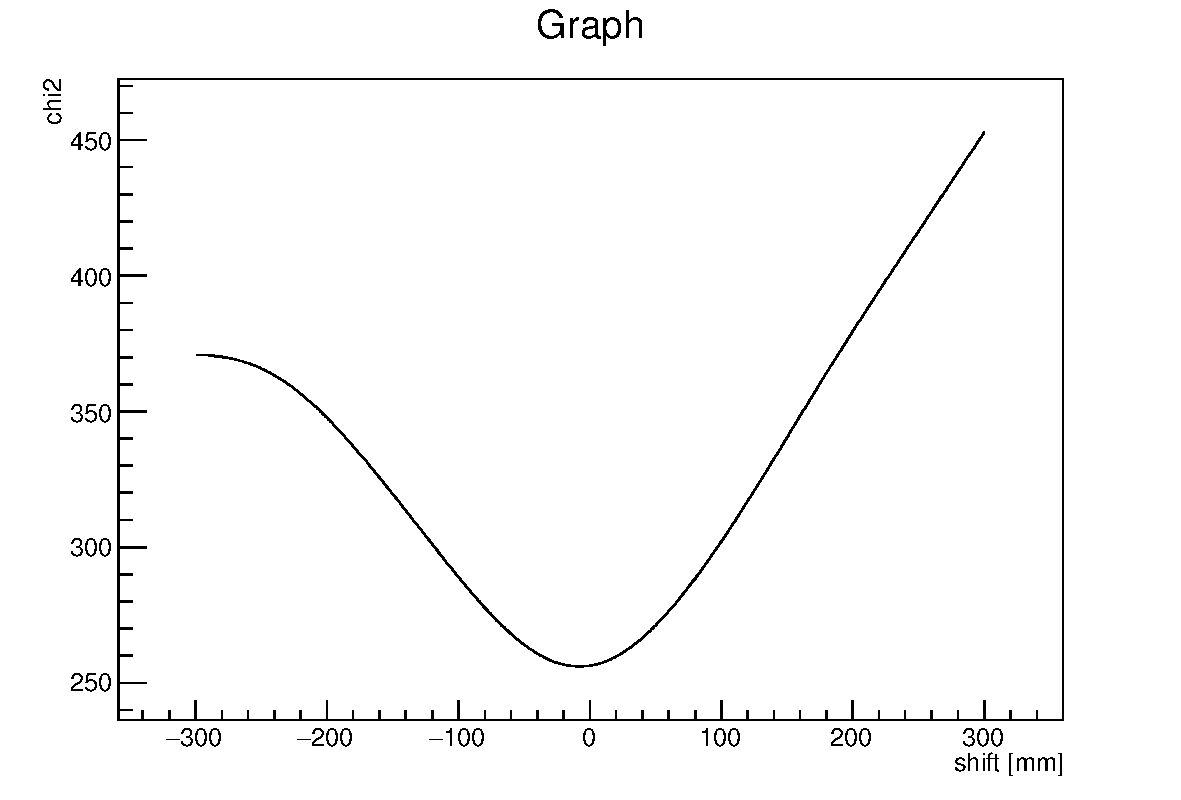
\includegraphics[width=0.33\textwidth]{./Figure/2017-08-02_Distribution_Chi2_1e8_LC.pdf}}
  \subfloat[\label{fig:fig_Results_Chi2_Distribution_Variation_CC_simulation_Hadronth_LC}]{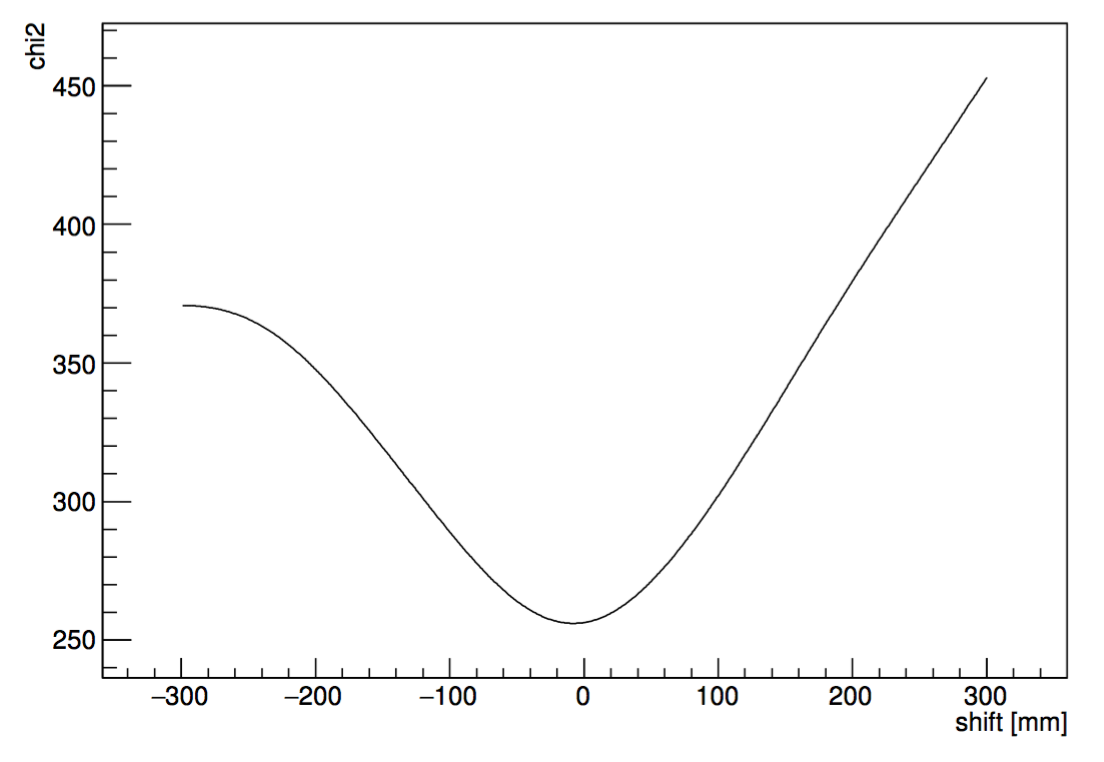
\includegraphics[width=0.33\textwidth]{./Figure/chi2_linecone.png}}
 %\subfloat[\label{fig:fig_Results_Chi2_Distribution_Variation_CC_simulation_Hadronth_MLEM}]{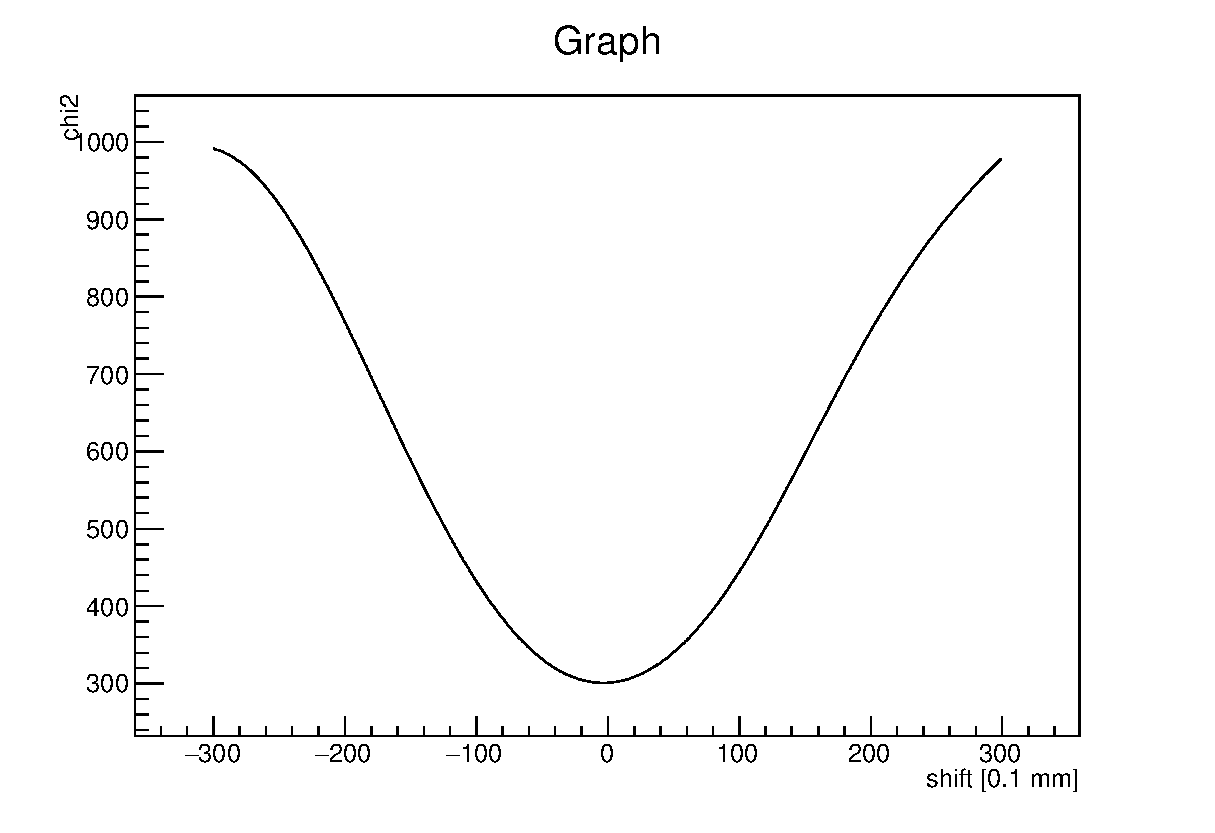
\includegraphics[width=0.33\textwidth]{./Figure/2017-08-02_Distribution_Chi2_Results_binning_1mm_ShiftNurbs0_1mm_1e8_article_MLEM.eps}}\\
 \subfloat[\label{fig:fig_Results_Chi2_Distribution_Variation_CC_simulation_Hadronth_MLEM}]{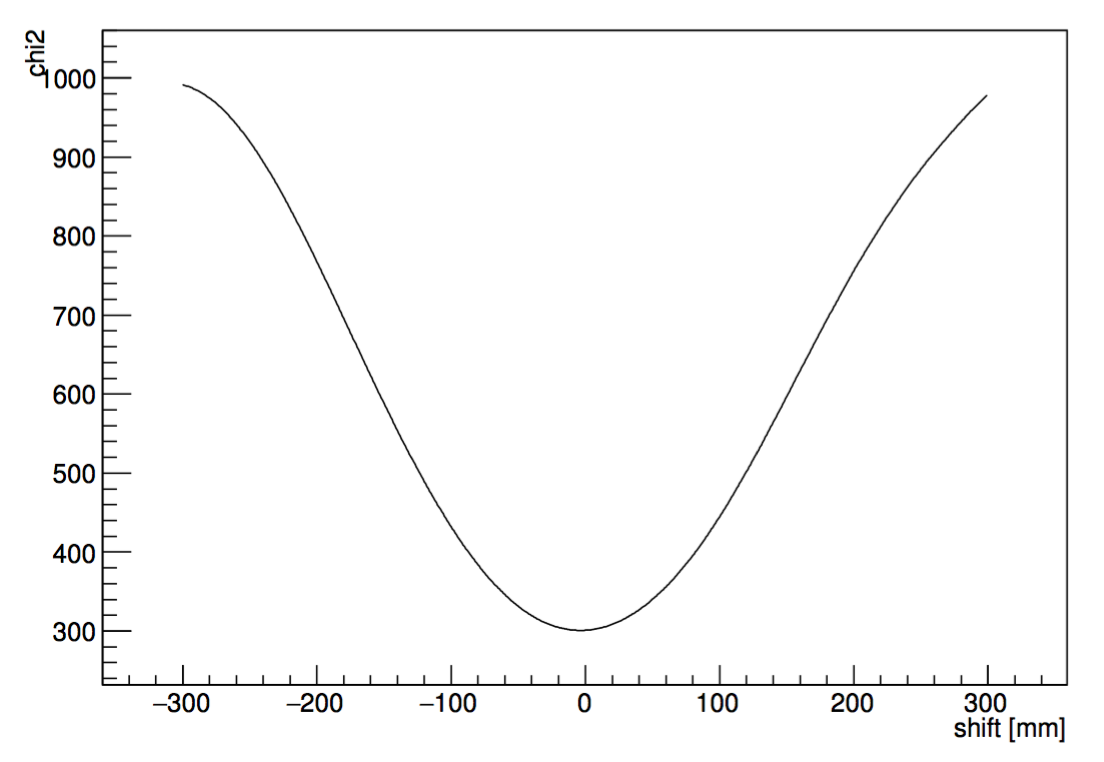
\includegraphics[width=0.33\textwidth]{./Figure/chi2_MLEM.png}}\\
  %\subfloat[\label{fig:fig_Results_Precision_Distribution_Variation_CC_simulation_Hadronth_LC} ]{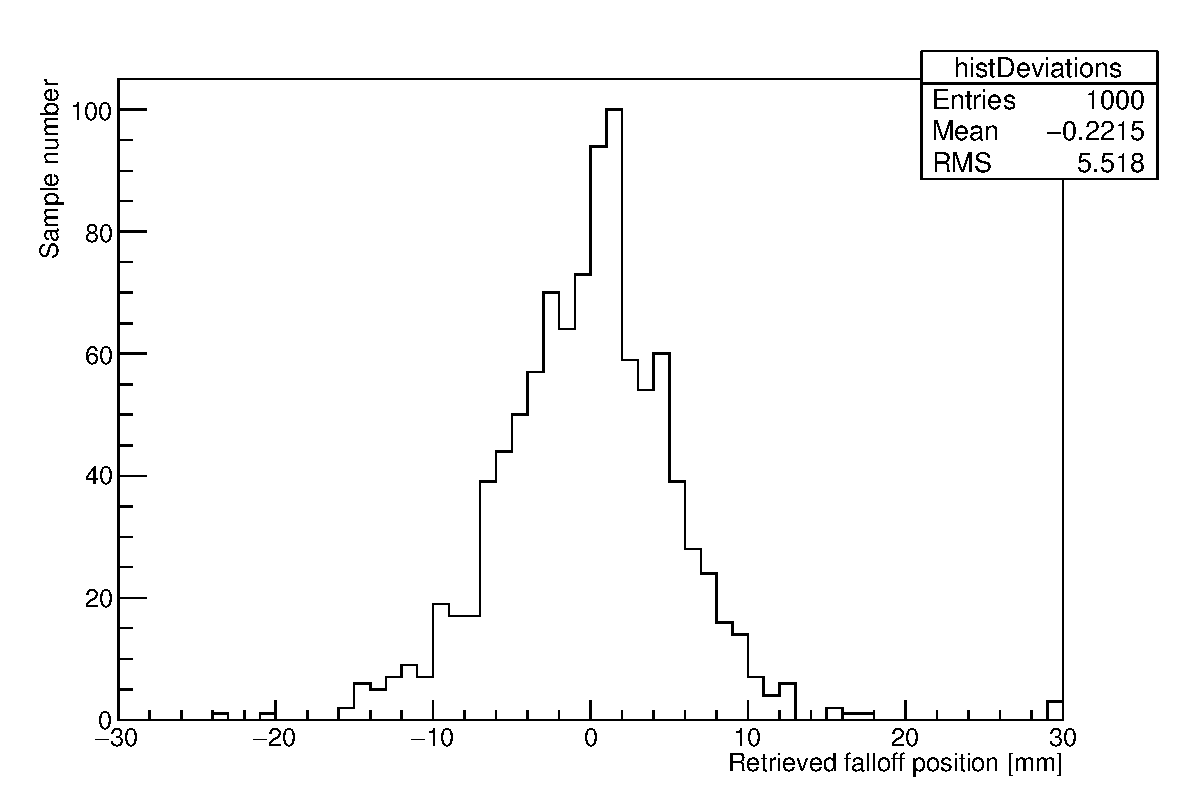
\includegraphics[width=0.33\textwidth]{./Figure/2017-08-02_Distribution_finale_1e8_Article_LC.pdf}}
  \subfloat[\label{fig:fig_Results_Precision_Distribution_Variation_CC_simulation_Hadronth_LC} ]{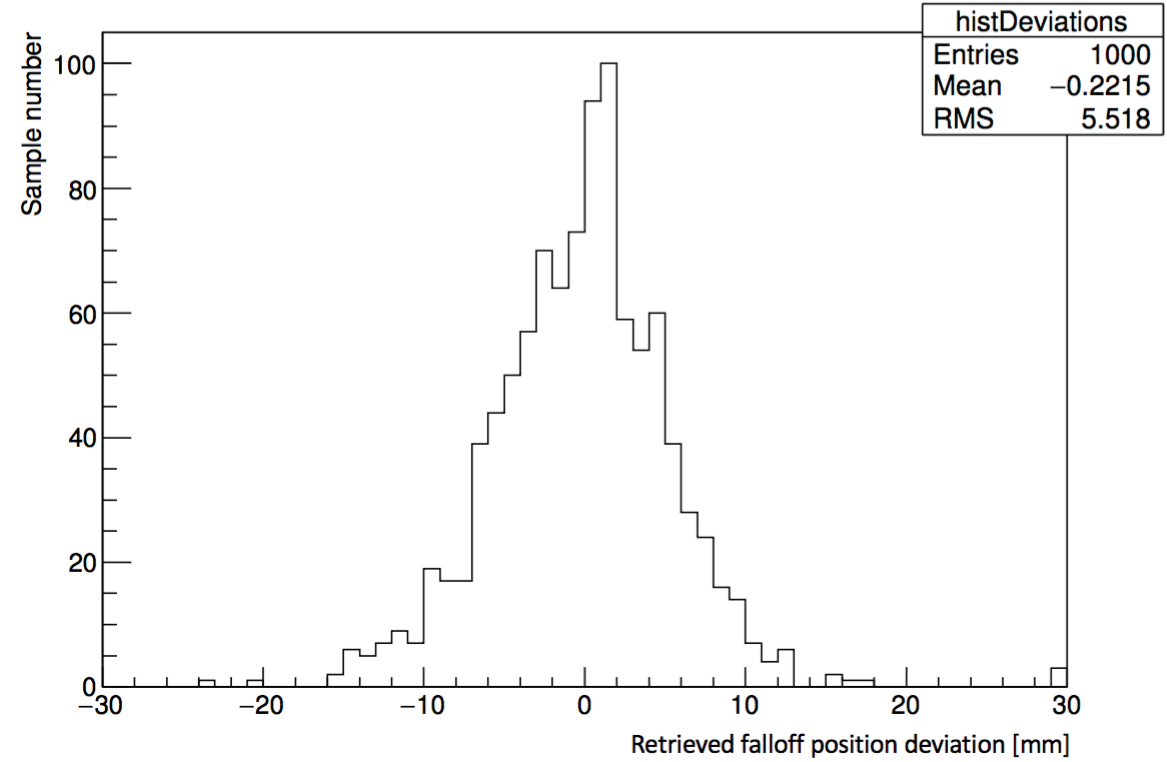
\includegraphics[width=0.33\textwidth]{./Figure/deviation_linecone.png}}
 %\subfloat[\label{fig:fig_Results_Precision_Distribution_Variation_CC_simulation_Hadronth_MLEM} ]{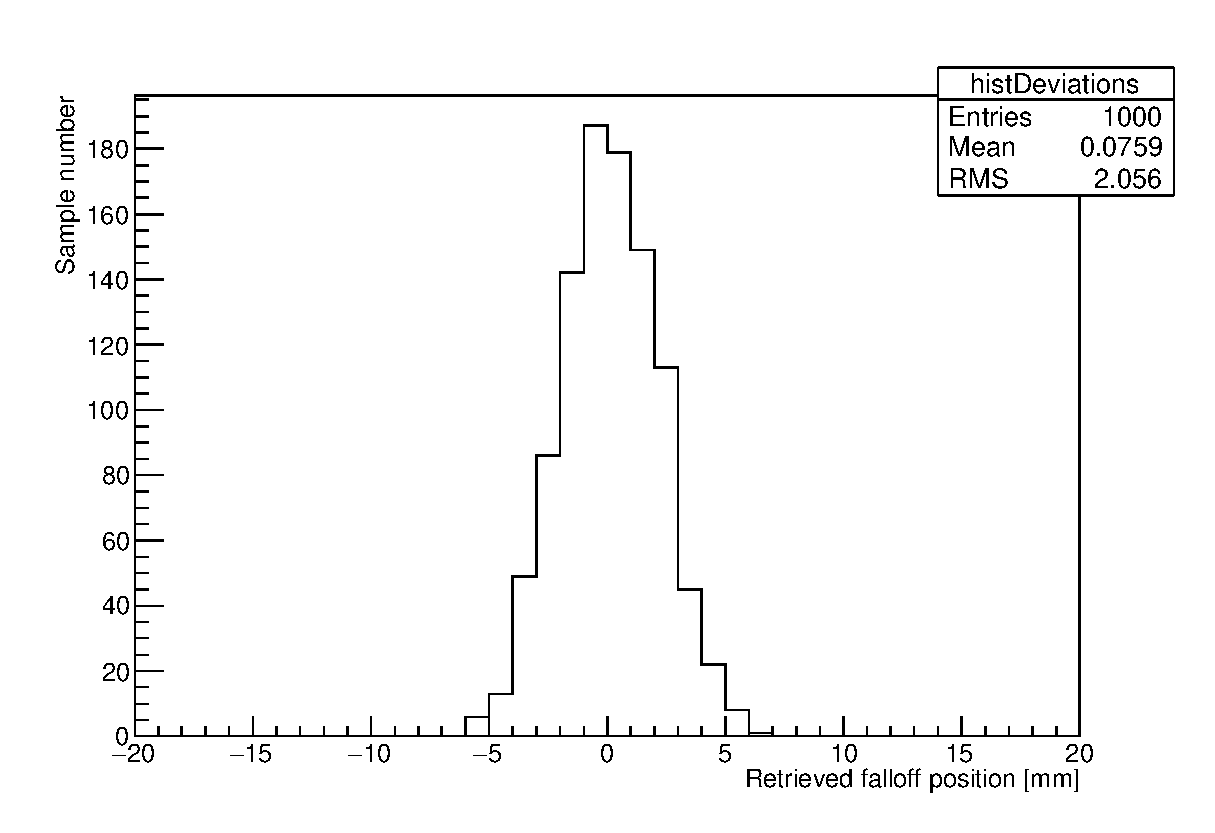
\includegraphics[width=0.33\textwidth]{./Figure/2017-08-02_FallOff_Results_binning_1mm_ShiftNurbs0_1mm_1e8_Article_MLEM.eps}}
 \subfloat[\label{fig:fig_Results_Precision_Distribution_Variation_CC_simulation_Hadronth_MLEM} ]{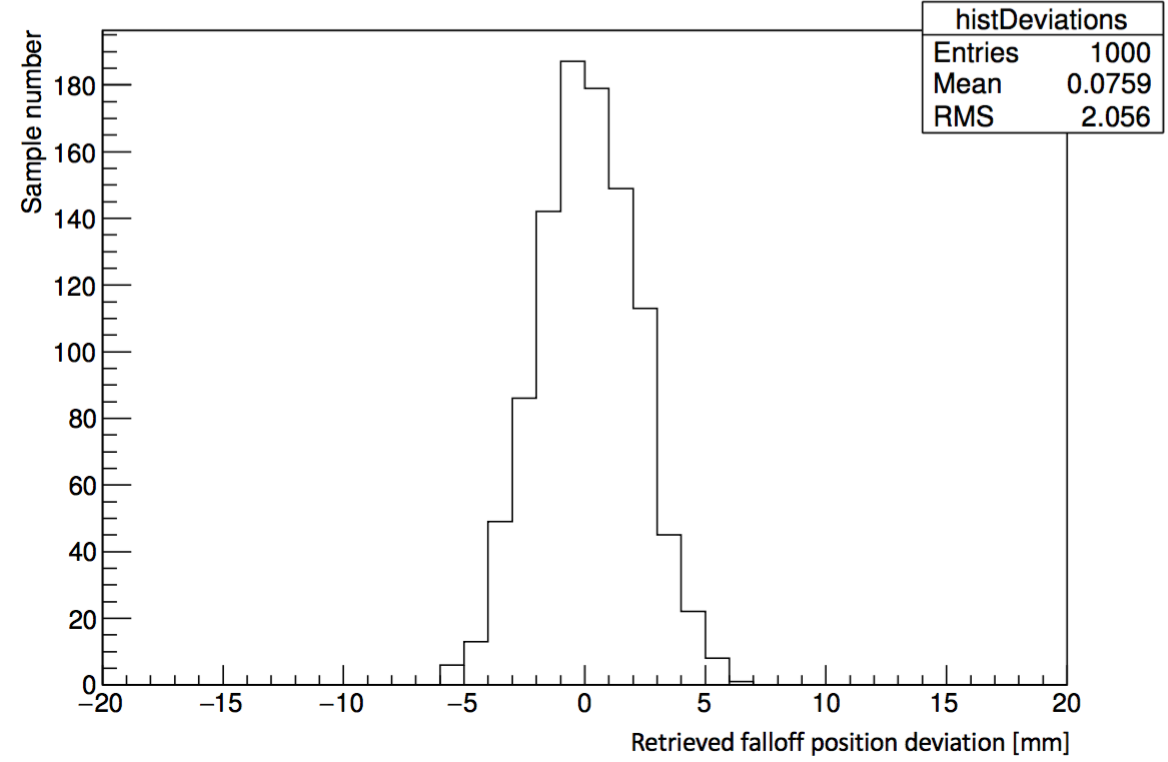
\includegraphics[width=0.33\textwidth]{./Figure/deviation_MLEM.png}}
\caption{Treatment comparison for the same proton simulation with the line cone algorithm (left column: figures \ref{fig:fig_Results_Estimation_Camera_Profil_highStat_CC_simulation_Hadronth_LineCone}, \ref{fig:fig_Estimation_Camera_CC_NURBS_Poisson_LC}, \ref{fig:fig_Results_Chi2_Distribution_Variation_CC_simulation_Hadronth_LC}, \ref{fig:fig_Results_Precision_Distribution_Variation_CC_simulation_Hadronth_LC}) and the LM-MLEM algorithm (right column: figures \ref{fig:fig_Results_Estimation_Camera_Profil_highStat_CC_simulation_Hadronth_MLEM}, \ref{fig:fig_Estimation_Camera_CC_NURBS_Poisson_MLEM}, \ref{fig:fig_Results_Chi2_Distribution_Variation_CC_simulation_Hadronth_MLEM}, \ref{fig:fig_Results_Precision_Distribution_Variation_CC_simulation_Hadronth_MLEM}). The first row gives the reconstructed profile for $2\times10^{10}$ incident protons (figure \ref{fig:fig_Results_Estimation_Camera_Profil_highStat_CC_simulation_Hadronth_LineCone}) and for $1\times10^{10}$ incident protons (figure \ref{fig:fig_Results_Estimation_Camera_Profil_highStat_CC_simulation_Hadronth_MLEM}) respectively. The figures \ref{fig:fig_Estimation_Camera_CC_NURBS_Poisson_LC} and \ref{fig:fig_Estimation_Camera_CC_NURBS_Poisson_MLEM} are showing the reference curve (blue) and the estimated curve with Poisson's law at $1\times10^8$ incident protons. The figures \ref{fig:fig_Results_Chi2_Distribution_Variation_CC_simulation_Hadronth_LC} and \ref{fig:fig_Results_Chi2_Distribution_Variation_CC_simulation_Hadronth_MLEM} are the $\chi^2$ minimization results for one realization. The minimum of the curve gives the best fit between the reference curve and the low statistics one. Finally, the figures  \ref{fig:fig_Results_Precision_Distribution_Variation_CC_simulation_Hadronth_LC} and \ref{fig:fig_Results_Precision_Distribution_Variation_CC_simulation_Hadronth_MLEM} represents the results for 1000 $\chi^2$ minimizations. The Compton camera precision is estimated thanks to the standard deviation of the distribution. }
\end{figure}

